%!TEX root = lecture_slides.tex
%%%%%%%%%%%%%%%%%%%%%%%%%%%%%%%%%%%%%%%%
%Some macros for diagrams of random variables
\def\RVraw{(-2.5,0) circle [radius=1.7]
	(-2.5,0) circle [radius=1.7]
	(2.5,0) circle [radius=1.7]
	node [above left] at (-3.75,1.25) {$S$}
	node [above right] at (3.75,1.25) {$\mathbb{R}$}
	node [above] at (0,2) {$X\colon S \mapsto \mathbb{R}$}}
%%%%%%%%%%%%%%%%%%%%%%%%%%%%%%%%%%%%%%%%
\begin{frame}
\frametitle{Recall: Properties of Probability Mass Functions}

If $p(x)$ is the pmf of a random variable $X$, then
\begin{enumerate}[(i)]
	\item $0\leq p(x) \leq 1$ for all $x$ \vspace{1em}
	\item $\displaystyle \sum_{\mbox{all } x} p(x) = 1$
\end{enumerate}

\vspace{0.75em}
where ``all $x$'' is shorthand for ``all $x$ in the support of $X$.''
\end{frame}
%%%%%%%%%%%%%%%%%%%%%%%%%%%%%%%%%%%%%%%%
\section{Cumulative Distribution Functions (CDFs)}
%%%%%%%%%%%%%%%%%%%%%%%%%%%%%%%%%%%%%%%%

\begin{frame}
\frametitle{Cumulative Distribution Function (CDF)}
\framesubtitle{This Def.\ is \alert{the same} for continuous RVs.}

The CDF gives the probability that a RV $X$ \alert{does not exceed} a specified threshold $x_0$, as a function of $x_0$
	$$F(x_0) = P(X \leq x_0)$$

\begin{alertblock}{Important!}
The threshold $x_0$ is allowed to be \emph{any real number}. In particular, it doesn't have to be in the support of $X$! 
\end{alertblock}

\end{frame}
%%%%%%%%%%%%%%%%%%%%%%%%%%%%%%%%%%%%%%%%
\begin{frame}
\frametitle{Discrete RVs: Sum the pmf to get the CDF}
\begin{center}
	\alert{$$\boxed{F(x_0) = \sum_{x\leq x_0} p(x)}$$}
\end{center}

\small
 
\begin{block}{Why?}
The events $\{X = x\}$ are mutually exclusive, so we sum to get the probability of their union for all $x\leq x_0$:
	$$F(x_0) = P(X \leq x_0)=   P\left(\bigcup_{x\leq x_0}\{X = x\}\right) =   \sum_{x \leq x_0} P(X = x) =   \sum_{x \leq x_0} p(x)$$
\end{block}

\end{frame}


%%%%%%%%%%%%%%%%%%%%%%%%%%%%%%%%%%%%%%%%

\begin{frame}[t]
	% \frametitle{Sum the pmf to get the CDF}
	% \framesubtitle{Coin-Flip Random Variable}

\begin{columns}[t]
	\column{0.48\textwidth}
	\begin{block}{Probability Mass Function}
	\begin{figure}
\centering
\begin{tikzpicture}[scale = 1.2]
\draw [<->] (0,2) node [above]{$p(x)$} -- (0,0) -- (3,0) node [right]{$x$};
\draw [blue, thick] (0.75,0) node [black, below]{0} -- (0.75,1.5);
\draw [blue, thick] (2.25,0) node [black, below]{1} -- (2.25,1.5);
\draw [dashed, gray] (0, 1.5) node [black, left]{$1/2$} -- (3,1.5);
\draw [fill=blue] (2.25,1.51) circle [radius = 0.05];
\draw [fill=blue] (0.75,1.51) circle [radius = 0.05];
\end{tikzpicture}
\end{figure}
\begin{eqnarray*}
	p(0) &=& 1/2\\
	p(1) &=& 1/2
\end{eqnarray*}
	\end{block}

	\column{0.48\textwidth}
	\begin{block}{Cumulative Dist.\ Function}
\begin{figure}
\centering
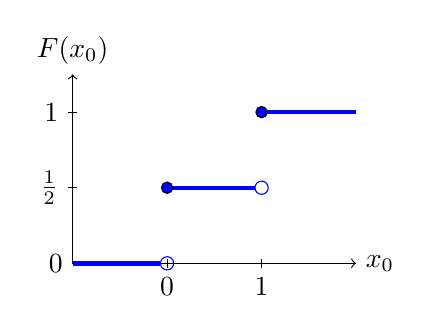
\begin{tikzpicture}[scale = 1.2]
\draw [<->] (0,2) node [above]{$F(x_0)$} -- (0,0) -- (3,0) node [right]{$x_0$};
\draw (-0.05, 1.6) node [black, left]{$1$} -- (0.05,1.6);
\draw (-0.05, 0.8) node [black, left]{$\frac{1}{2}$} -- (0.05,0.8);
\draw [blue, ultra thick] (0,0) -- (0.93,0);
\draw [blue, ultra thick] (1,0.8) -- (1.93,0.8);
\draw [blue, ultra thick] (2,1.6) -- (3,1.6);
\draw (1,-0.05) node [black, below]{0} -- (1,0.05);
\draw (2,-0.05) node [black, below]{1} -- (2,0.05);
\draw (0,0) node [black, left]{$0$};
\draw [blue] (1,0) circle [radius = 0.07];
\draw [fill = blue] (1,0.8) circle [radius = 0.06];
\draw [blue] (2,0.8) circle [radius = 0.07];
\draw [fill = blue] (2,1.6) circle [radius = 0.06];
\end{tikzpicture}
\end{figure}
\begin{eqnarray*}
	F(x_0) = \left\{\begin{array}{ll} 0,& x_0 < 0\\ \frac{1}{2}, &0\leq x_0 < 1\\ 1,& x_0 \geq 1\end{array}\right.
\end{eqnarray*}
	\end{block}
\end{columns}
\end{frame}

%%%%%%%%%%%%%%%%%%%%%%%%%%%%%%%%%%%%%%%%

\begin{frame}
\frametitle{Properties of CDFs}
\framesubtitle{These are also true for continuous RVs.}
	\begin{enumerate}
		\item $\lim_{x_0 \rightarrow \infty} F(x_0) = 1$
		\item $\lim_{x_0 \rightarrow -\infty} F(x_0) = 0$
		\item Non-decreasing: $x_0 < x_1 \Rightarrow F(x_0)\leq F(x_1)$
		\item Right-continuous (``open'' versus ``closed'' on prev.\ slide)
	\end{enumerate}
	
	
	 
	
	
\vspace{1em}
\begin{alertblock}{Since $F(x_0) = P(X\leq x_0)$,  we have $0\leq F(x_0)\leq 1$ for all $x_0$}\end{alertblock}
\end{frame}
%%%%%%%%%%%%%%%%%%%%%%%%%%%%%%%%%%%%%%%%
\section{The Bernoulli Random Variable}
%%%%%%%%%%%%%%%%%%%%%%%%%%%%%%%%%%%%%%%%
\begin{frame}
\frametitle{Bernoulli Random Variable -- Generalization of Coin Flip}
\small
\begin{block}{Support Set}
$\{0,1\}$ -- 1 traditionally called ``success,'' 0 ``failure''
\end{block}

\begin{block}{Probability Mass Function}
	\begin{eqnarray*}
		p(0) &=& 1-p\\
		p(1) &=& p
	\end{eqnarray*}

	\begin{block}{Cumulative Distribution Function}
\begin{eqnarray*}
	F(x_0) = \left\{\begin{array}{ll} 0,& x_0 < 0\\ 1-p, &0\leq x_0 < 1\\ 1,& x_0 \geq 1\end{array}\right.
\end{eqnarray*}
\end{block}
\end{block}

\end{frame}
%%%%%%%%%%%%%%%%%%%%%%%%%%%%%%%%%%%%%%%%
\begin{frame}
	\frametitle{\href{http://fditraglia.shinyapps.io/binom_cdf/}{http://fditraglia.shinyapps.io/binom\_cdf/}}
\framesubtitle{Set the second slider to 1 and play around with the others.}

\begin{figure}
	\fbox{\includegraphics[scale = 0.2]{./images/binom_cdf_screenshot}}
\end{figure}

\end{frame}


%%%%%%%%%%%%%%%%%%%%%%%%%%%%%%%%%%%%%%%%
\section{Definition of Expected Value}
%%%%%%%%%%%%%%%%%%%%%%%%%%%%%%%%%%%%%%%%
\begin{frame}
\frametitle{Average Winnings Per Trial \hfill \includegraphics[scale = 0.05]{./images/clicker}}
If the realizations of the coin-flip RV were \alert{payoffs}, how much would you expect to win per play \emph{on average} in a long sequence of plays?
$$X = \left\{ \begin{array}{l}  \$0, \mbox{Tails}\\ \$1, \mbox{Heads}\end{array} \right.$$
\end{frame}
%%%%%%%%%%%%%%%%%%%%%%%%%%%%%%%%%%%%%%%%
\begin{frame}
\frametitle{Expected Value (aka Expectation)}
The expected value of a discrete RV $X$ is given by
	$$E[X] = \sum_{\mbox{all} \; x} x \cdot p(x)$$

  \vspace{1em}
  \alert{In other words, the expected value of a discrete RV is the \emph{probability-weighted average of its realizations}.}

  \vspace{1em}

  \begin{block}{Notation}
    We sometimes write $\mu$ as shorthand for $E[X]$.  \end{block}
\end{frame}
%%%%%%%%%%%%%%%%%%%%%%%%%%%%%%%%%%%%%%%%
\begin{frame}
  \frametitle{Expected Value of Bernoulli RV}
$$X = \left\{ \begin{array}{l}  0, \mbox{Failure: } 1-p\\ 1, \mbox{Success: } p\end{array} \right.$$

\vspace{2em}
 
$$\sum_{\mbox{all} \; x} x \cdot p(x) = 0 \cdot (1-p) + 1 \cdot p = p$$
\end{frame}
%%%%%%%%%%%%%%%%%%%%%%%%%%%%%%%%%%%%%%%%
\begin{frame}
  \frametitle{Your Turn to Calculate an Expected Value \hfill\includegraphics[scale = 0.05]{./images/clicker}}
  Let $X$ be a random variable with support set $\left\{ 1,2,3 \right\}$ where $p(1)=p(2)=1/3$. Calculate $E[X]$.

  \pause

  \vspace{1em}
  \begin{equation*}
    E[X] = \sum_{\mbox{all }x} x \cdot p(x) = 1 \times 1/3 + 2 \times 1/3 + 3 \times 1/3 = 2
  \end{equation*}
\end{frame}
%%%%%%%%%%%%%%%%%%%%%%%%%%%%%%%%%%%%%%%%

\begin{frame}
\frametitle{Random Variables and Parameters}



\begin{block}{Notation: $X \sim$ Bernoulli$(p)$}
Means $X$ is a Bernoulli RV with $P(X = 1) = p$ and $P(X= 0) = 1-p$. The tilde is read ``distributes as.''

\end{block}


\begin{block}{Parameter}
Any constant that appears in the definition of a RV, here $p$. 
\end{block}


\end{frame}
%%%%%%%%%%%%%%%%%%%%%%%%%%%%%%%%%%%%%%%%

\begin{frame}
\frametitle{Constants Versus Random Variables}

 \alert{This is a crucial distinction that students sometimes miss:}
 \vspace{1em}
 

 		\begin{block}{Random Variables}
 			\begin{itemize}
 			\item Suppose $X$ is a RV -- the values it takes on are random
 			\item A function $g(X)$ of a RV is itself a RV as we'll learn today.
 			\end{itemize}
 		\end{block}
 
 		\begin{block}{Constants}
 			\begin{itemize}
 				\item $E[X]$ is a constant (you should convince yourself of this)
 				\item Realizations $x$ are constants. What is random is \emph{which} realization the RV takes on.
 				\item Parameters are constants (e.g.\ $p$ for Bernoulli RV)
 				\item Sample size $n$ is a constant
 			\end{itemize}
 		\end{block} 

\end{frame}
%%%%%%%%%%%%%%%%%%%%%%%%%%%%%%%%%%%%%%%%
\section{Expected Value of a Function}
%%%%%%%%%%%%%%%%%%%%%%%%%%%%%%%%%%%%%%%%
\begin{frame}
\Huge \centering The St.\ Petersburg Game

\end{frame}
%%%%%%%%%%%%%%%%%%%%%%%%%%%%%%%%%%%%%%%%
\begin{frame}
\frametitle{How Much Would You Pay?\hfill \includegraphics[scale = 0.05]{./images/clicker}}
How much would you be willing to pay for the right to play the following game?

\vspace{1em}
\begin{quote}
Imagine a fair coin. The coin is tossed once. If it falls heads, you receive a prize of \$2 and the game stops. If not, it is tossed again. If it falls heads on the second toss, you get \$4 and the game stops. If not, it is tossed again. If it falls heads on the third toss, you get \$8 and the game stops, and so on. The game stops after the first head is thrown. If the first head is thrown on the $x^{th}$ toss, the prize is \$$2^x$
\end{quote}

\end{frame}
%%%%%%%%%%%%%%%%%%%%%%%%%%%%%%%%%%%%%%%%
\begin{frame}
\frametitle{$X =$ Trial Number of First Head}
\begin{table}
\begin{tabular}{c|c|c|c}
	$x$ & $2^x$ & $p(x)$& $2^x \cdot p(x)$\\
		\hline \uncover<2->{
	1&2&1/2&1\\
	2&4&1/4&1\\
	3&8&1/8&1\\}\uncover<3->{
	$\vdots$&$\vdots$&$\vdots$&$\vdots$\\
	n&$2^n$&$1/2^n$&1\\
	$\vdots$&$\vdots$&$\vdots$&$\vdots$}
\end{tabular}
\end{table}
$$E[Y] = \sum_{\mbox{all } x} 2^x\cdot p(x) = \uncover<4->{1 + 1 + 1 + \hdots}\uncover<5->{ = \infty}$$
\end{frame}
%%%%%%%%%%%%%%%%%%%%%%%%%%%%%%%%%%%%%%%%

\begin{frame}
\begin{center}
\Huge Functions of Random Variables are Themselves Random Variables
\end{center}

\end{frame}
%%%%%%%%%%%%%%%%%%%%%%%%%%%%%%%%%%%%%%%%
\begin{frame}
  \frametitle{Example: $X\sim \mbox{Bernoulli}(p)$, $Y = (X+1)^2$}

\begin{block}{Support Set for $Y$} \pause
$\{(0 + 1)^2, (1 + 1)^2\} =\{1, 4\}$
\end{block}

\begin{block}{Probability Mass Function for $Y$} \pause
	$$p_Y(y) = \left\{\begin{array}{ll} 1-p& y = 1\\ p& y = 4\\ 0& \mbox{otherwise}\end{array}\right.$$
\end{block}

\pause
\begin{block}{Expected Value of $Y$}
  \[
    \sum_{y\in \left\{ 1,4 \right\}} y \times p_Y(y) \pause = 1 \times (1 - p )  + 4 \times p \pause = 1 + 3p
  \]
\end{block}

\end{frame}
%%%%%%%%%%%%%%%%%%%%%%%%%%%%%%%%%%%%%%%%
\begin{frame}
  \frametitle{Example: $X\sim \mbox{Bernoulli}(p)$, $Y = (X+1)^2$}


  \begin{block}{$E[g(X)] = E[(X+1)^2]$}
  \[
    \sum_{y\in \left\{ 1,4 \right\}} y \times p_Y(y)  = 1 \times (1 - p )  + 4 \times p  = 1 + 3p
  \]
\end{block}

\pause

\begin{block}{$g(E[X]) = (E[X] + 1)^2$}
  \[\left(E[X] + 1\right)^2 = (p + 1)^2 = 1 + 2p + p^2\]
\end{block}

\pause

\begin{alertblock}{In general: $1 + 3p \neq 1 + 2p + p^2$!}
\end{alertblock}

\end{frame}
%%%%%%%%%%%%%%%%%%%%%%%%%%%%%%%%%%%%%%%%


\begin{frame}
\huge $$E[g(X)] \neq g(E[X])$$
\begin{center}
	\large (Expected value of Function $\neq$ Function of Expected Value)
\end{center}


\end{frame}
%%%%%%%%%%%%%%%%%%%%%%%%%%%%%%%%%%%%%%%%

\begin{frame}
\frametitle{Expectation of a Function of a Discrete RV}
Let $X$ be a random variable and $g$ be a function. Then:
$$\boxed{E[g(X)] = \sum_{\mbox{all } x} g(x) p(x)}$$


 \alert{This is how we proceeded in the St.\ Petersburg Game Example}
\end{frame}
%%%%%%%%%%%%%%%%%%%%%%%%%%%%%%%%%%%%%%%%
\begin{frame}
\frametitle{Your Turn: Calculate $E[X^2]$ \hfill \includegraphics[scale = 0.05]{./images/clicker}}
$X$ has support $\{-1, 0, 1\}$, $p(-1) = p(0) = p(1) = 1/3$.
\pause

\begin{eqnarray*}
 E[X^2] &=&  \sum_{\mbox{all } x} x^2 p(x) = \sum_{x \in \{-1, 0, 1\}} x^2 p(x) \\ \\ \pause
 	&=& (-1)^2 \cdot (1/3) + (0)^2 \cdot (1/3) + (1)^2 \cdot (1/3)\\ \pause
 	&=& 1/3 + 1/3\\ 
 	&=& 2/3 \approx 0.67
\end{eqnarray*}

\end{frame}
%%%%%%%%%%%%%%%%%%%%%%%%%%%%%%%%%%%%%%%%
\begin{frame}[fragile]
  \footnotesize
\begin{knitrout}
\definecolor{shadecolor}{rgb}{0.969, 0.969, 0.969}\color{fgcolor}\begin{kframe}
\begin{alltt}
\hlkwd{set.seed}\hlstd{(}\hlnum{794729}\hlstd{)}
\hlstd{sims} \hlkwb{<-} \hlkwd{sample}\hlstd{(}\hlkwd{c}\hlstd{(}\hlopt{-}\hlnum{1}\hlstd{,} \hlnum{0}\hlstd{,} \hlnum{1}\hlstd{),} \hlkwc{size} \hlstd{=} \hlnum{1e6}\hlstd{,} \hlkwc{replace} \hlstd{=} \hlnum{TRUE}\hlstd{,}
               \hlkwc{prob} \hlstd{=} \hlkwd{c}\hlstd{(}\hlnum{1}\hlopt{/}\hlnum{3}\hlstd{,} \hlnum{1}\hlopt{/}\hlnum{3}\hlstd{,} \hlnum{1}\hlopt{/}\hlnum{3}\hlstd{))}
\hlkwd{head}\hlstd{(sims)}
\end{alltt}
\begin{verbatim}
## [1]  1 -1  0  0  1  1
\end{verbatim}
\begin{alltt}
\hlkwd{mean}\hlstd{(sims)}
\end{alltt}
\begin{verbatim}
## [1] -0.001182
\end{verbatim}
\begin{alltt}
\hlkwd{mean}\hlstd{(sims}\hlopt{^}\hlnum{2}\hlstd{)}
\end{alltt}
\begin{verbatim}
## [1] 0.66682
\end{verbatim}
\end{kframe}
\end{knitrout}

\end{frame}

%%%%%%%%%%%%%%%%%%%%%%%%%%%%%%%%%%%%%%%%
\section{Linearity of Expectation}
%%%%%%%%%%%%%%%%%%%%%%%%%%%%%%%%%%%%%%%%

\begin{frame}
\frametitle{Linearity of Expectation}
\framesubtitle{Holds for Continuous RVs as well, but proof is different.}
Let $X$ be a RV and $a,b$ be constants. Then:
	$$E[a + bX] = a + bE[X]$$

  \begin{alertblock}{This is a Crucial Exception}
    In general $E[g(X)]$ does not equal $g(E[X])$.
    But in the special case where $g$ is a \alert{linear function}, $g(X) = a + bX$, the two \alert{are equal}.
\end{alertblock}
\end{frame}
%%%%%%%%%%%%%%%%%%%%%%%%%%%%%%%%%%%%%%%%
\begin{frame}
\frametitle{Example: Linearity of Expectation \hfill \includegraphics[scale = 0.05]{./images/clicker} }
Let $X \sim \mbox{Bernoulli}(1/3)$ and define $Y = 3X + 2$
\vspace{1em}

\begin{enumerate}
  \item What is $E[X]$? \pause \hspace{2em} \alert{$E[X] = 0 \times 2/3 + 1 \times 1/3 = 1/3$} \pause
  \item What is $E[Y]$? \pause \hspace{2em} \alert{$E[Y] = E[3X + 2] = 3E[X] + 2 = 3$}
\end{enumerate}
\end{frame}
%%%%%%%%%%%%%%%%%%%%%%%%%%%%%%%%%%%%%%%%

\begin{frame}
\frametitle{Proof: Linearity of Expectation For Discrete RV}

\begin{eqnarray*}
	E[a + bX] &=& \sum_{\mbox{all } x}  (a + bx) p(x)\\ \\
	 &=&  \sum_{\mbox{all } x} p(x) \cdot a + \sum_{\mbox{all } x}p(x) \cdot bx\\ \\
	&=&  a\sum_{\mbox{all } x} p(x) + b\sum_{\mbox{all } x} x \cdot p(x) \\ \\
	&=&  a + b E[X]
\end{eqnarray*}


\end{frame}
%%%%%%%%%%%%%%%%%%%%%%%%%%%%%%%%%%%%%%%%
